\begin{problem}{3.2.5}
  Show that the map $f(x) = (x - 1/x)/2$, $x \neq 0$, has no fixed points but it has
  period 2-points. Find the 2-cycle, and by looking at the graph of $f^3 (x)$, check to see
  whether or not it has a 3-cycle. Why does this not contradict Sharkovsky’s Theorem?
\end{problem}

\begin{proof}The function $f$ will have a fixed point if and only if the function $g(x) = f(x) - x$
  has real roots. We see that
  \begin{align*}
    g(x) = f(x) - x = \frac{x^2-1}{2x} - x = -\frac{x^2+1}{2x} = 0
  \end{align*}
  if and only if $x^2 + 1 =0$. Thus, $g$ has no real roots and $f$ has no fixed points.

  If $h(x) = f^2(x) - x$ has real solutions, then these solutions give rise to a 2-cycle of $f$.
  Thus,
  \begin{align*}
    h(x) = f(f(x)) - x = \frac{\left(\frac{x^2-1}{2x}\right)^2-1}{2\left(\frac{x^2-1}{2x}\right)} - x
    = -\frac{- 3 x^4 - 2 x^2 + 1}{-4x^3 + 4 x}= 0
  \end{align*}
  if and only if $- 3 x^4 - 2 x^2 + 1=0$, the real solutions of which are given by $3^{-1/2}$ and $-3^{-1/2}$.
  Hence, $\{3^{-1/2}, -3^{-1/2}\}$ is a 2-cycle of $f$.

  The graphs of $f^3(x)$ and $y=x$ are shown in Figure 1. From these graphs we see that
  the graph of $f^3(x)$ crosses the line $y=x$ at 6 points. Since $f$ has a 2-cycle, 2 of these points
  arise from the fact that the solutions of $f^2(x) = x$ also satisfy $f^3(x) = x$. However, of the four remaining
  points, the graph of $f^3(x)$ does not cross the graph $y=x$ at exactly 3 points so a 3-cycle does not arise for $f(x)$.

  \begin{figure}[!h]
    \centerline{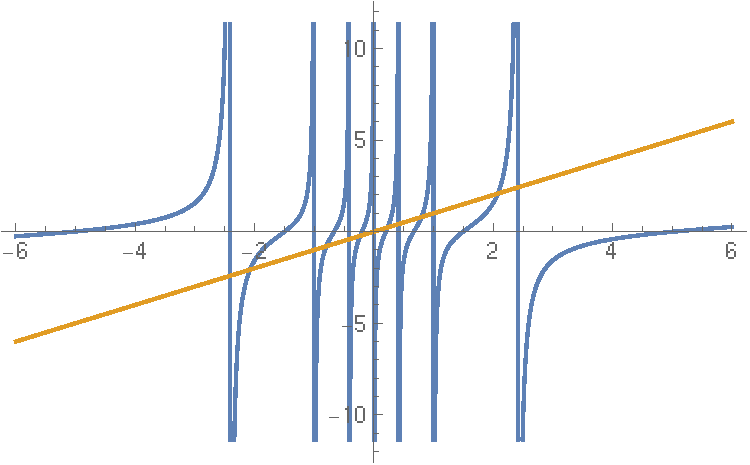
\includegraphics[scale=0.9]{no_3_cycle}}
    \caption{The graphs of $f^3(x)$ (blue) and $y=x$ (orange).}
  \end{figure}


  Note that the domain of $f$ is given by $(-\infty, 0) \cup (0, \infty)$. Since the domain of $f$ is
  not an interval, it does not satisfy the assumptions of Sharkovsky's Theorem
  and thus the theorem does not apply.

\end{proof}
\newpage
